    \documentclass[12pt,a4paper]{article}
    \usepackage[T2A]{fontenc}
    \usepackage[utf8]{inputenc}
    \usepackage[russian]{babel}
    \usepackage{amsmath}
    \usepackage{amssymb}
    \usepackage{graphicx}
    \usepackage{floatrow}
    \usepackage{booktabs}
    \usepackage{wrapfig}
    \usepackage{lipsum}
    \usepackage{subcaption}
    \usepackage{fancyhdr}
    \usepackage{mathrsfs}
    \usepackage{tikz}

    \usepackage{graphicx, scalerel}
    \usepackage[warn]{mathtext}
    \usepackage{indentfirst}
    \usepackage[margin = 25mm]{geometry}
    \usepackage{caption}
    \usepackage{multirow}
    \usepackage{gensymb}
    
    \newcommand{\figref}[1]{(См. рис. \ref{#1})}
    \newcommand{\secref}[1]{(См. раздел. \ref{#1})}
    
    \newcommand{\e}[1]{\text{$\cdot10^{#1}$}}
    
    \pagestyle{fancy}
    \fancyhead{}
    \fancyhead[L]{Работа 4.3.3}
    \fancyhead[R]{}
    \fancyfoot[C]{\thepage}
    
    \author{\normalsize Выполнил: Голубович Тимур, группа Б01-108 \\
    	\normalsize 04.05.2023}
    \date{}
    
    \usepackage{float}
    \restylefloat{table}
    \title{
    	\large Отчет о выполнении лабораторной работы 4.3.3 \\
    	\Large Исследование разрешающей способности микроскопа методом Аббе
     }
    
    \begin{document}
    	\maketitle
    	
    \section*{Цель работы}
    Определение дифракционного предела разрешения обёектива методом Аббе.
    
    \section*{Оборудование и приборы} 
    Лазер;
    кассета с набором сеток разного периода;
    линзы;
    щель с микрометрическим винтом;
    оптический стол с набором рейтеров и крепёжных винтов;
    экран;
    линейка.

	
    \section*{Теоретическое введение}

    Для иммерсионного микроскопа разрешающая способность объектива при некогерентном
    освещении
    
    \begin{equation}
    \ell_{\min } \approx \frac{0.61 \lambda}{n \sin u}
    \end{equation}
    
    где $u-$ апертурный угол объектива микроскопа (угол между оптической осью и лучом, направленным из центра объекта в край линзы).
    Метод Аббе для оценки разрешающей способности состоит в разделении хода лучей на две части: сначала рассматривается картина в задней фокальной плоскости $F$ объектива. Она называется первичным изображением или фурье-образом. Это первичное изображение рассматривается как источник волн (принцип Гюйгенса-Френеля), создающий изображение в плоскости $P_{2}$, сопряжённой плоскости предмета - вторичное изображение. Первичное изображение есть картина дифракции Фраунгофера (на дифракционной решётке), если её период $d$, то для направления максимальной интенсивности $\varphi_{m}$
    
    \begin{equation}
    d \sin \varphi_{m}=m \lambda
    \end{equation}
    
    При этом проходят пучки только с $\varphi_{m}<u .$ Можно условием разрешения считать, что $u>\varphi_{1}$, иначе говоря
    
    \begin{equation}
    \sin u \geq \lambda / d
    \end{equation}
    
    Или
    
    \begin{equation}
    d \geq \frac{\lambda}{\sin u} \approx \frac{\lambda}{D / 2 f}
    \end{equation}
    
    где $D-$ диаметр линзы, $f-$ фокусное расстояние. Двумерную решётку можно рассматривать как две перпендикулярные друг другу, для максимумов которых выполняется соотношение
    
    \begin{equation}
        d \sin \varphi_{x}=m_{x} \lambda, \quad d \sin \varphi_{y}=m_{y} \lambda
    \end{equation}


 
	\section*{Экспериментальная установка}

    \begin{figure}[h!]
    	\centering
    	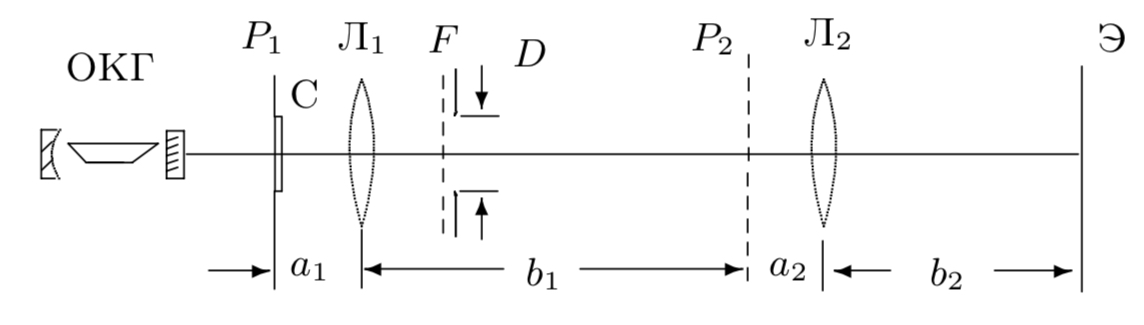
\includegraphics[width=\linewidth]{res/scheme}
    	\caption{Экспериментальная установка}
    	\label{lab}
    \end{figure}
    
    Схема установки приведена на Рис. 1. Предметом $P_{1}$ служат сетки в кассете $C .$ \\Линза Л1 -- длиннофокусная, а Л2 -- короткофокусная. В фокальную плоскость F устанавливаются диафрагмы D. С помощью сеток с разными $d$ и щелевой диафрагмы можно проверить третье соотношение. Период сеток может быть измерен либо по расстоянию между дифракционными максимумами на экране, либо по увеличенному с помощью микроскопа изображению сетки на экране. Пространственную фильтрацию (получение наклонного изображение решётки) можно получить с помощью подбора угла наклона и ширины вспомогательной щели.


 
    \section*{Ход работы}
	
	\begin{center}
		\textbf{I. Определение периода решёток по их пространственному спектру}
	\end{center}

    Соберём установку согласно описанию. Длина волны излучения лазера $\lambda=532$ нм.
    Расстояние от сетки до экрана $L=120 \pm 2$ см, погрешность объясняется неопределённостью положения сетки внутри кассеты, погрешностью меток на столе, использованных при измерении, и погрешностью прямого измерения. Измерим линейкой на экране расстояние $\Delta x$ между $n+1$ максимумами и рассчитаем по второй формуле с учётом $\varphi=\frac{\Delta x}{H}$ период решетки $d = \frac{n\lambda}{\Delta x}L$. Результаты приведены в Таблице $1 .$
    



        \begin{table}[h!]
    	   \centering
    	   \footnotesize
    	   \begin{tabular}{cccc}
\toprule
Номер решётки & $\Delta n$, дел & $\Delta x$, см & $d$, мкм \\
\midrule
1 & 4  & 19.9 & 12.83 \\
2 & 11 & 26.4 & 26.60 \\
3 & 21 & 26.5 & 50.59 \\
4 & 4  & 19.6 & 13.03 \\
5 & 11 & 26.5 & 26.50 \\
6 & 19 & 23.7 & 51.18 \\
\bottomrule
\end{tabular}

    	   \caption{Измерения периода решёток}
    	   \label{tab:t1}
        \end{table}
        
		\begin{figure}[H]
			\centering
			\includegraphics[width=0.5\linewidth]{src/hair.png}
			\caption{Дифракция на волосе}
		\end{figure}

    Также определим диаметр человеческого волоса с помощью дифракции. Для этого измеряем ширину его главного максимума ${\Delta l}_{\text{волоса}} = 1.1 \text{см}$. Рассчитаем диаметр волоса по формуле \ref{eq:hair}.

    \begin{equation}
        D_\text{волоса} = \frac{\lambda \cdot L}{{\Delta l}_{\text{волоса}}} = 58  \text{ мкм}.
        \label{eq:hair}
    \end{equation}


	\begin{center}
		\textbf{II. Определение периода решёток по изображению, увеличенному с помощью модели микроскопа}
	\end{center}

    Соберём модель микроскопа, добавив линзы согласно Рис. 1. Фокусные расстояния линз $F_{1}=  110$ мм, $F_{2}= 25$ мм. Измеряем необходимые расстояния:
        $$
        \begin{aligned}
        a_{1} &= 15  \pm 1 \text{ cм}, \\
        a_{2}+b_{1} &= 45 \pm 1 \text{ см}, \\
        b_{2} &= 74 \pm 1 \text{ см},
        \end{aligned}
        $$
    Погрешности здесь обусловлены неточностями в положениях сеток и линз. Из формулы тонкой линзы \fbox{$a_{2}=\frac{b_{2} F_{2}}{b_{2}-F_{2}}=24$ мм}, откуда \fbox{$a_{2} \approx F_{2}$}, поэтому в дальнейшем будем использовать это значение, следовательно $b_{1}= 42\pm 1$ см.  Увеличение микроскопа \fbox{$ \Gamma=\frac{b_{1} b_{2}}{a_{1} a_{2}}=87 \pm 10 .$}
    Повторим измерения периодов изображений в новой конфигурации, погрешности считаются аналогично. Измерение представлены в Таблице $2 .$
    Здесь $d$ определялось по формуле $d=\frac{\Delta x}{\Gamma n}$. Обратим внимание, что значения периодов решётки совпадают в пределах погрешности.


        \begin{table}[h!]
           \centering
           \footnotesize
           \begin{tabular}{cccc}
\toprule
Номер решётки & $\Delta n$, дел & $\Delta x$, см & $d$, мкм \\
\midrule
1 & 4  & 19.9 & 12.83 \\
2 & 11 & 26.4 & 26.60 \\
3 & 21 & 26.5 & 50.59 \\
4 & 4  & 19.6 & 13.03 \\
5 & 11 & 26.5 & 26.50 \\
6 & 19 & 23.7 & 51.18 \\
\bottomrule
\end{tabular}

           \caption{Измерения увеличенного изображение сетки}
           \label{tab:t2}
        \end{table}
    


	\begin{center}
		\textbf{III. Определение периода решёток по оценке разрешающей способности микроскопа}
	\end{center}

    Поместим в фокальной плоскости линзы $\text{Л}_{1}$ щелевую диафрагму с микрометрическим винтом и определим минимальную толщину $D$ при которой на экране видна двумерная решётка. В этом случае период будет вычисляться по формуле (3) в предельном случае
    
        \begin{equation}
            d=\frac{2 \lambda F_{1}}{D}
        \end{equation}
    
    погрешность вычисляется по формуле
    $$
    \sigma_{d}=d \frac{\sigma_{D}}{D} .
    $$
    Результаты приведены в Таблице $3 .$

        \begin{table}[h!]
           \centering
           \footnotesize
           \begin{tabular}{cccc}
\toprule
Номер решётки & $\Delta n$, дел & $\Delta x$, см & $d$, мкм \\
\midrule
1 & 4  & 19.9 & 12.83 \\
2 & 11 & 26.4 & 26.60 \\
3 & 21 & 26.5 & 50.59 \\
4 & 4  & 19.6 & 13.03 \\
5 & 11 & 26.5 & 26.50 \\
6 & 19 & 23.7 & 51.18 \\
\bottomrule
\end{tabular}

           \caption{Измерения разрешающей способности сеток}
           \label{tab:t3}
        \end{table}

    Через щель проходили только нулевой (по центру) и два первых максимумы, за исключением второй щели, где нулевой максимум был помещён к краю щели. Для первой решётки
    период таким методом измерить не получилось, так как ширины щели не хватает.
    Для проверки теории Аббе построим график $d=f\left(\frac{1}{D}\right)$ со значениями $d$ из части 1, погрешность $\frac{1}{D}$ рассчитывается по формуле
    
    $$
        \sigma_{1 / D}=\frac{\sigma_{D}}{D^{2}}
    $$
    
		\begin{figure}[H]
			\centering
			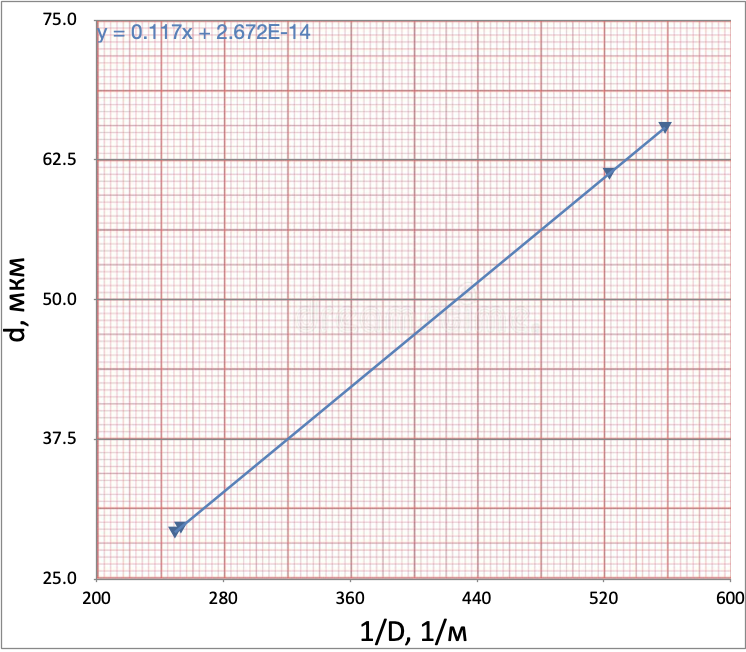
\includegraphics[width=0.8\linewidth]{src/plot.png}
			\caption{Зависимость $d\left( \frac{1}{D} \right)$}
		\end{figure}

    Угловой коэффициент прямой из $\text{MHK}\ k=(117 \pm 8) \cdot 10^{-9} {\text{м}}^{2}$, в пределах погрешности он совпадает с теоретическим $2 \lambda F_{1}= 106\cdot 10^{-9} {\text{ м}}^{2} .$ Таким образом, теория Аббе подтвердилась. 



	\begin{center}
		\textbf{IV. Пространственная фильтрация и мультиплицирование}
	\end{center}


    Для наблюдения фильтрации на сетке 2 откроем щель так, чтобы она пропускала только максимум нулевого порядка и, поворачивая щель, наблюдаем за изменением картины. Картины представлены на рисунках ниже. \\

    Измеряем периоды интерференционных полос: у горизонтальной щели $2 \; \frac{\text{полос}}{\text{см}}$, у вертикальнойй $2 \; \frac{\text{полос}} {\text{см}}$, у щели, повернутой на $45^{\circ}$ -- $2.7 \; \frac{\text{полос}}{\text{см}}$.

\begin{minipage}{0.47\textwidth}
\begin{center}
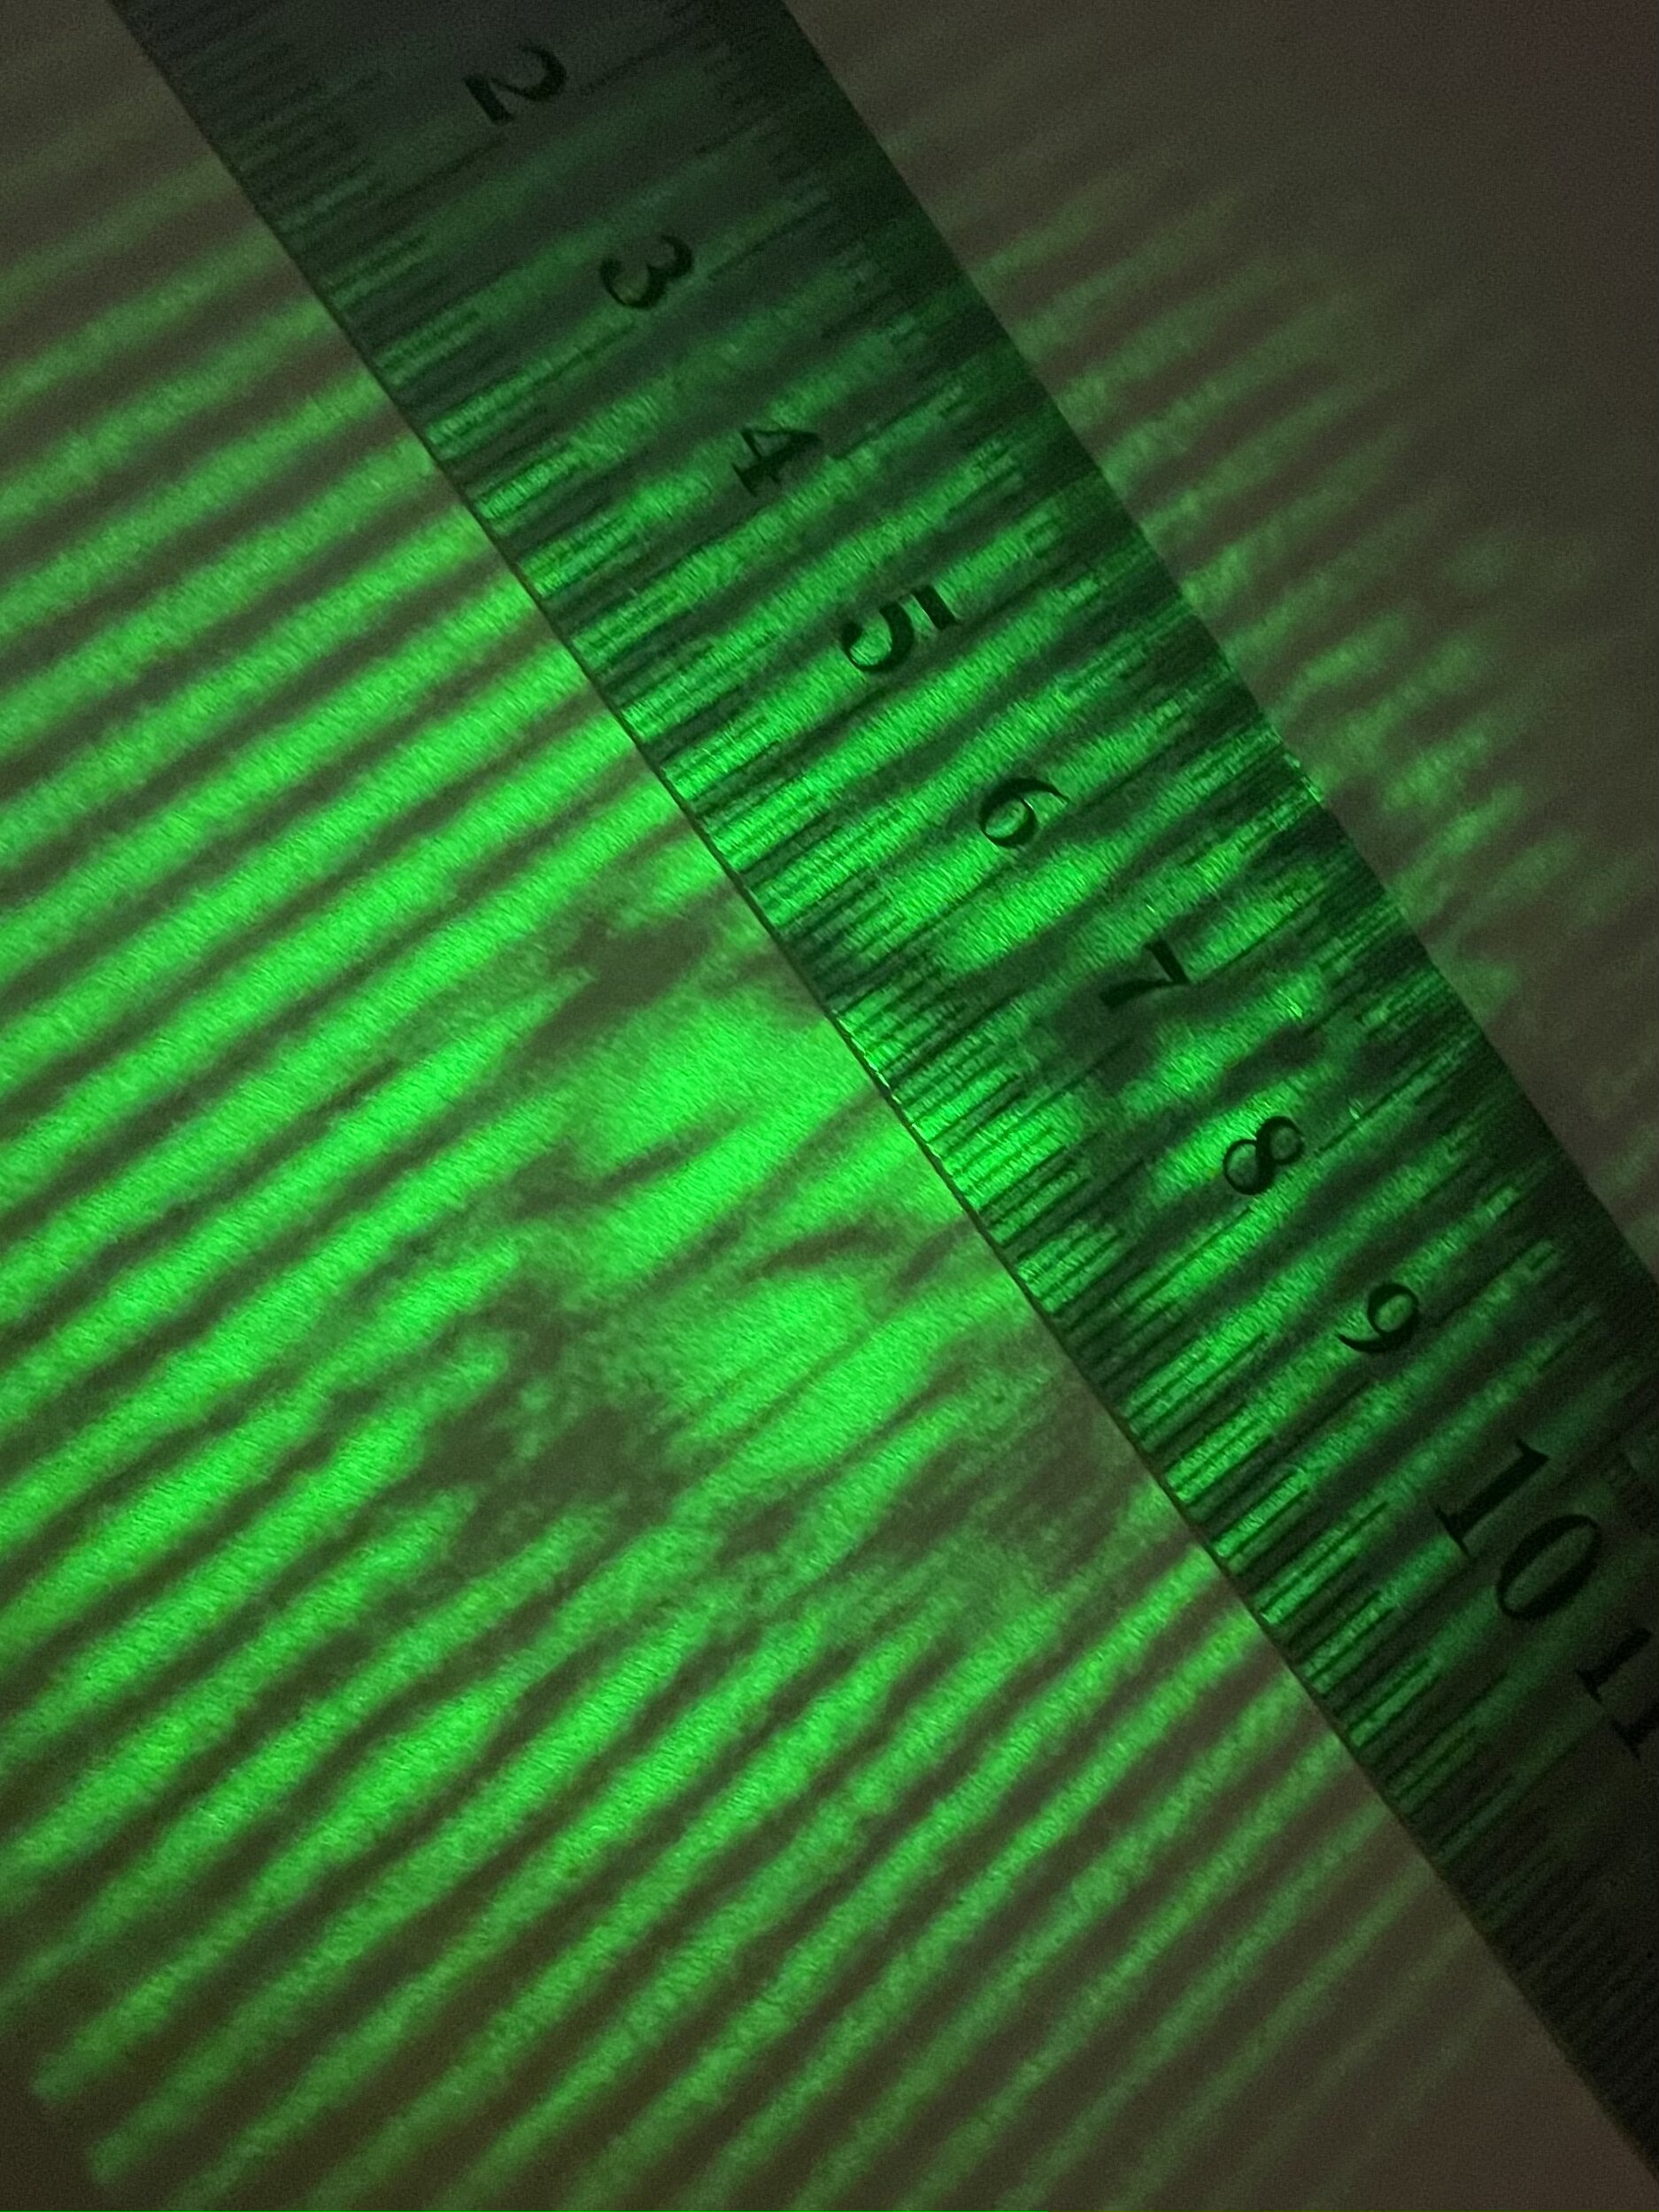
\includegraphics[width = \textwidth]{src/45.jpeg}
\end{center}

\begin{center}
Щель, повернутая на $45^{\circ}$
\end{center}
\end{minipage}
\begin{minipage}{0.47\textwidth}
\begin{center}
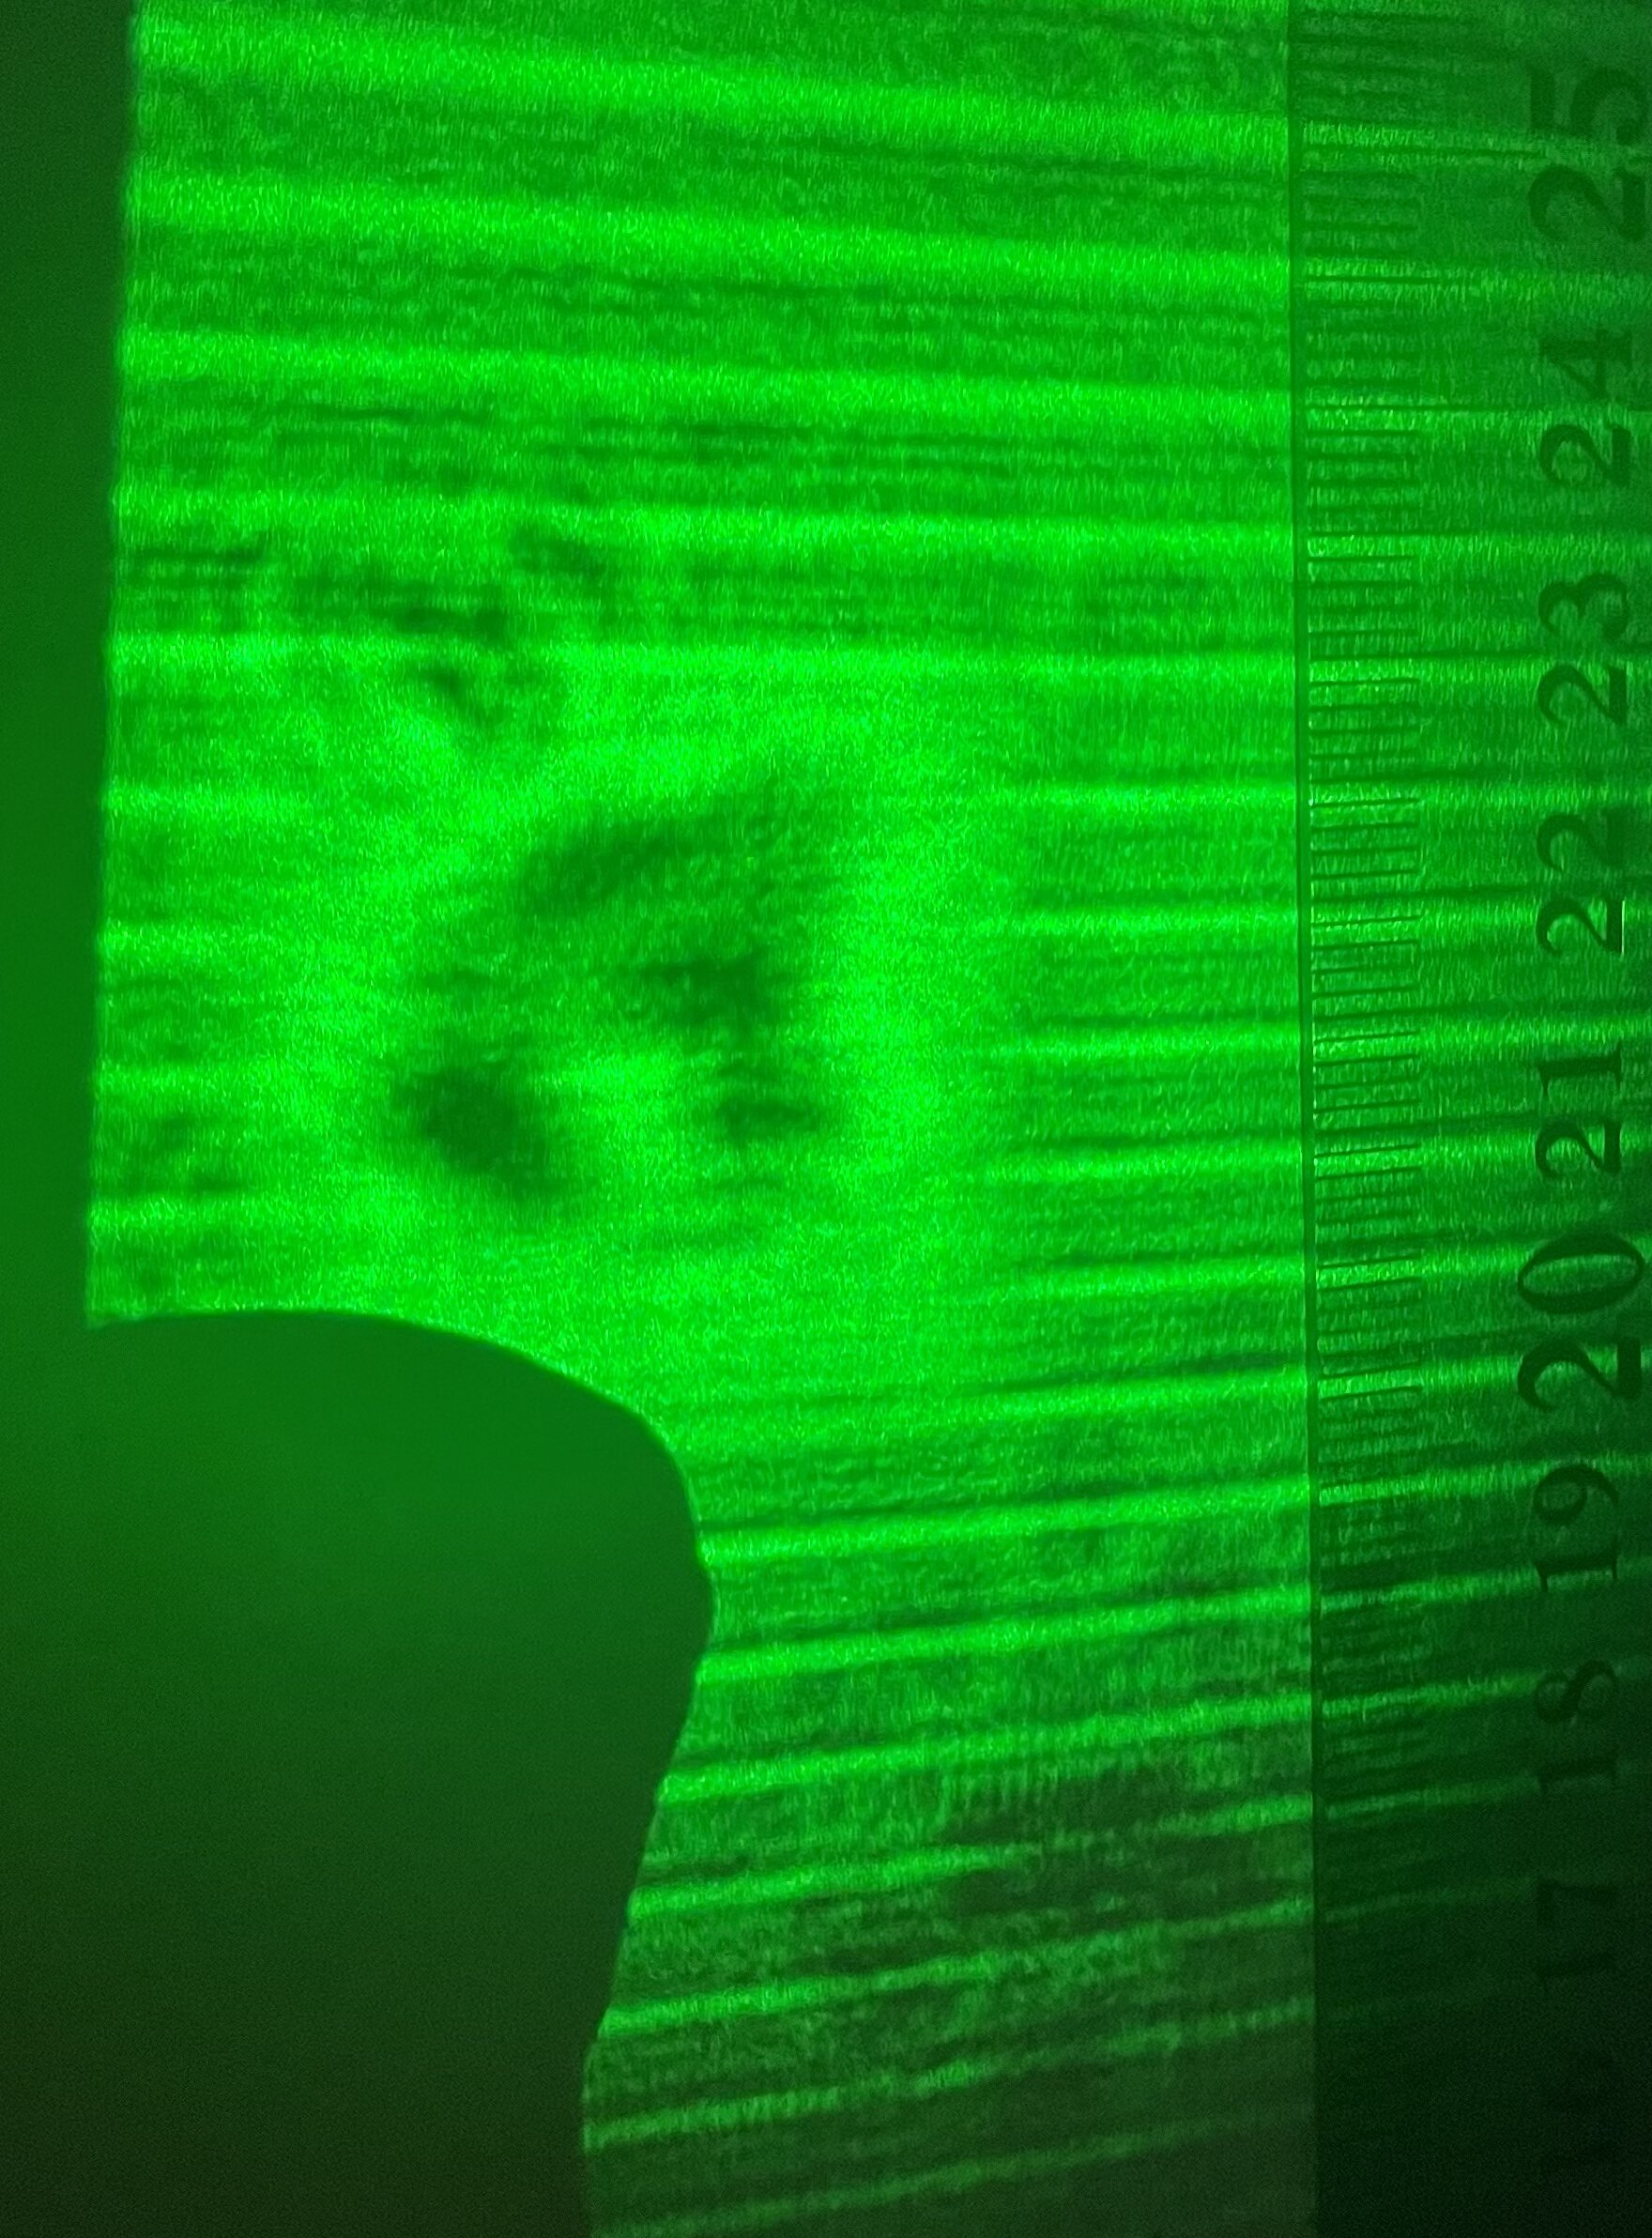
\includegraphics[width = 0.95\textwidth]{src/ver.jpeg}
\end{center}

\begin{center}
Вертикальная щель
\end{center}
\end{minipage}

		\begin{figure}
			\centering
			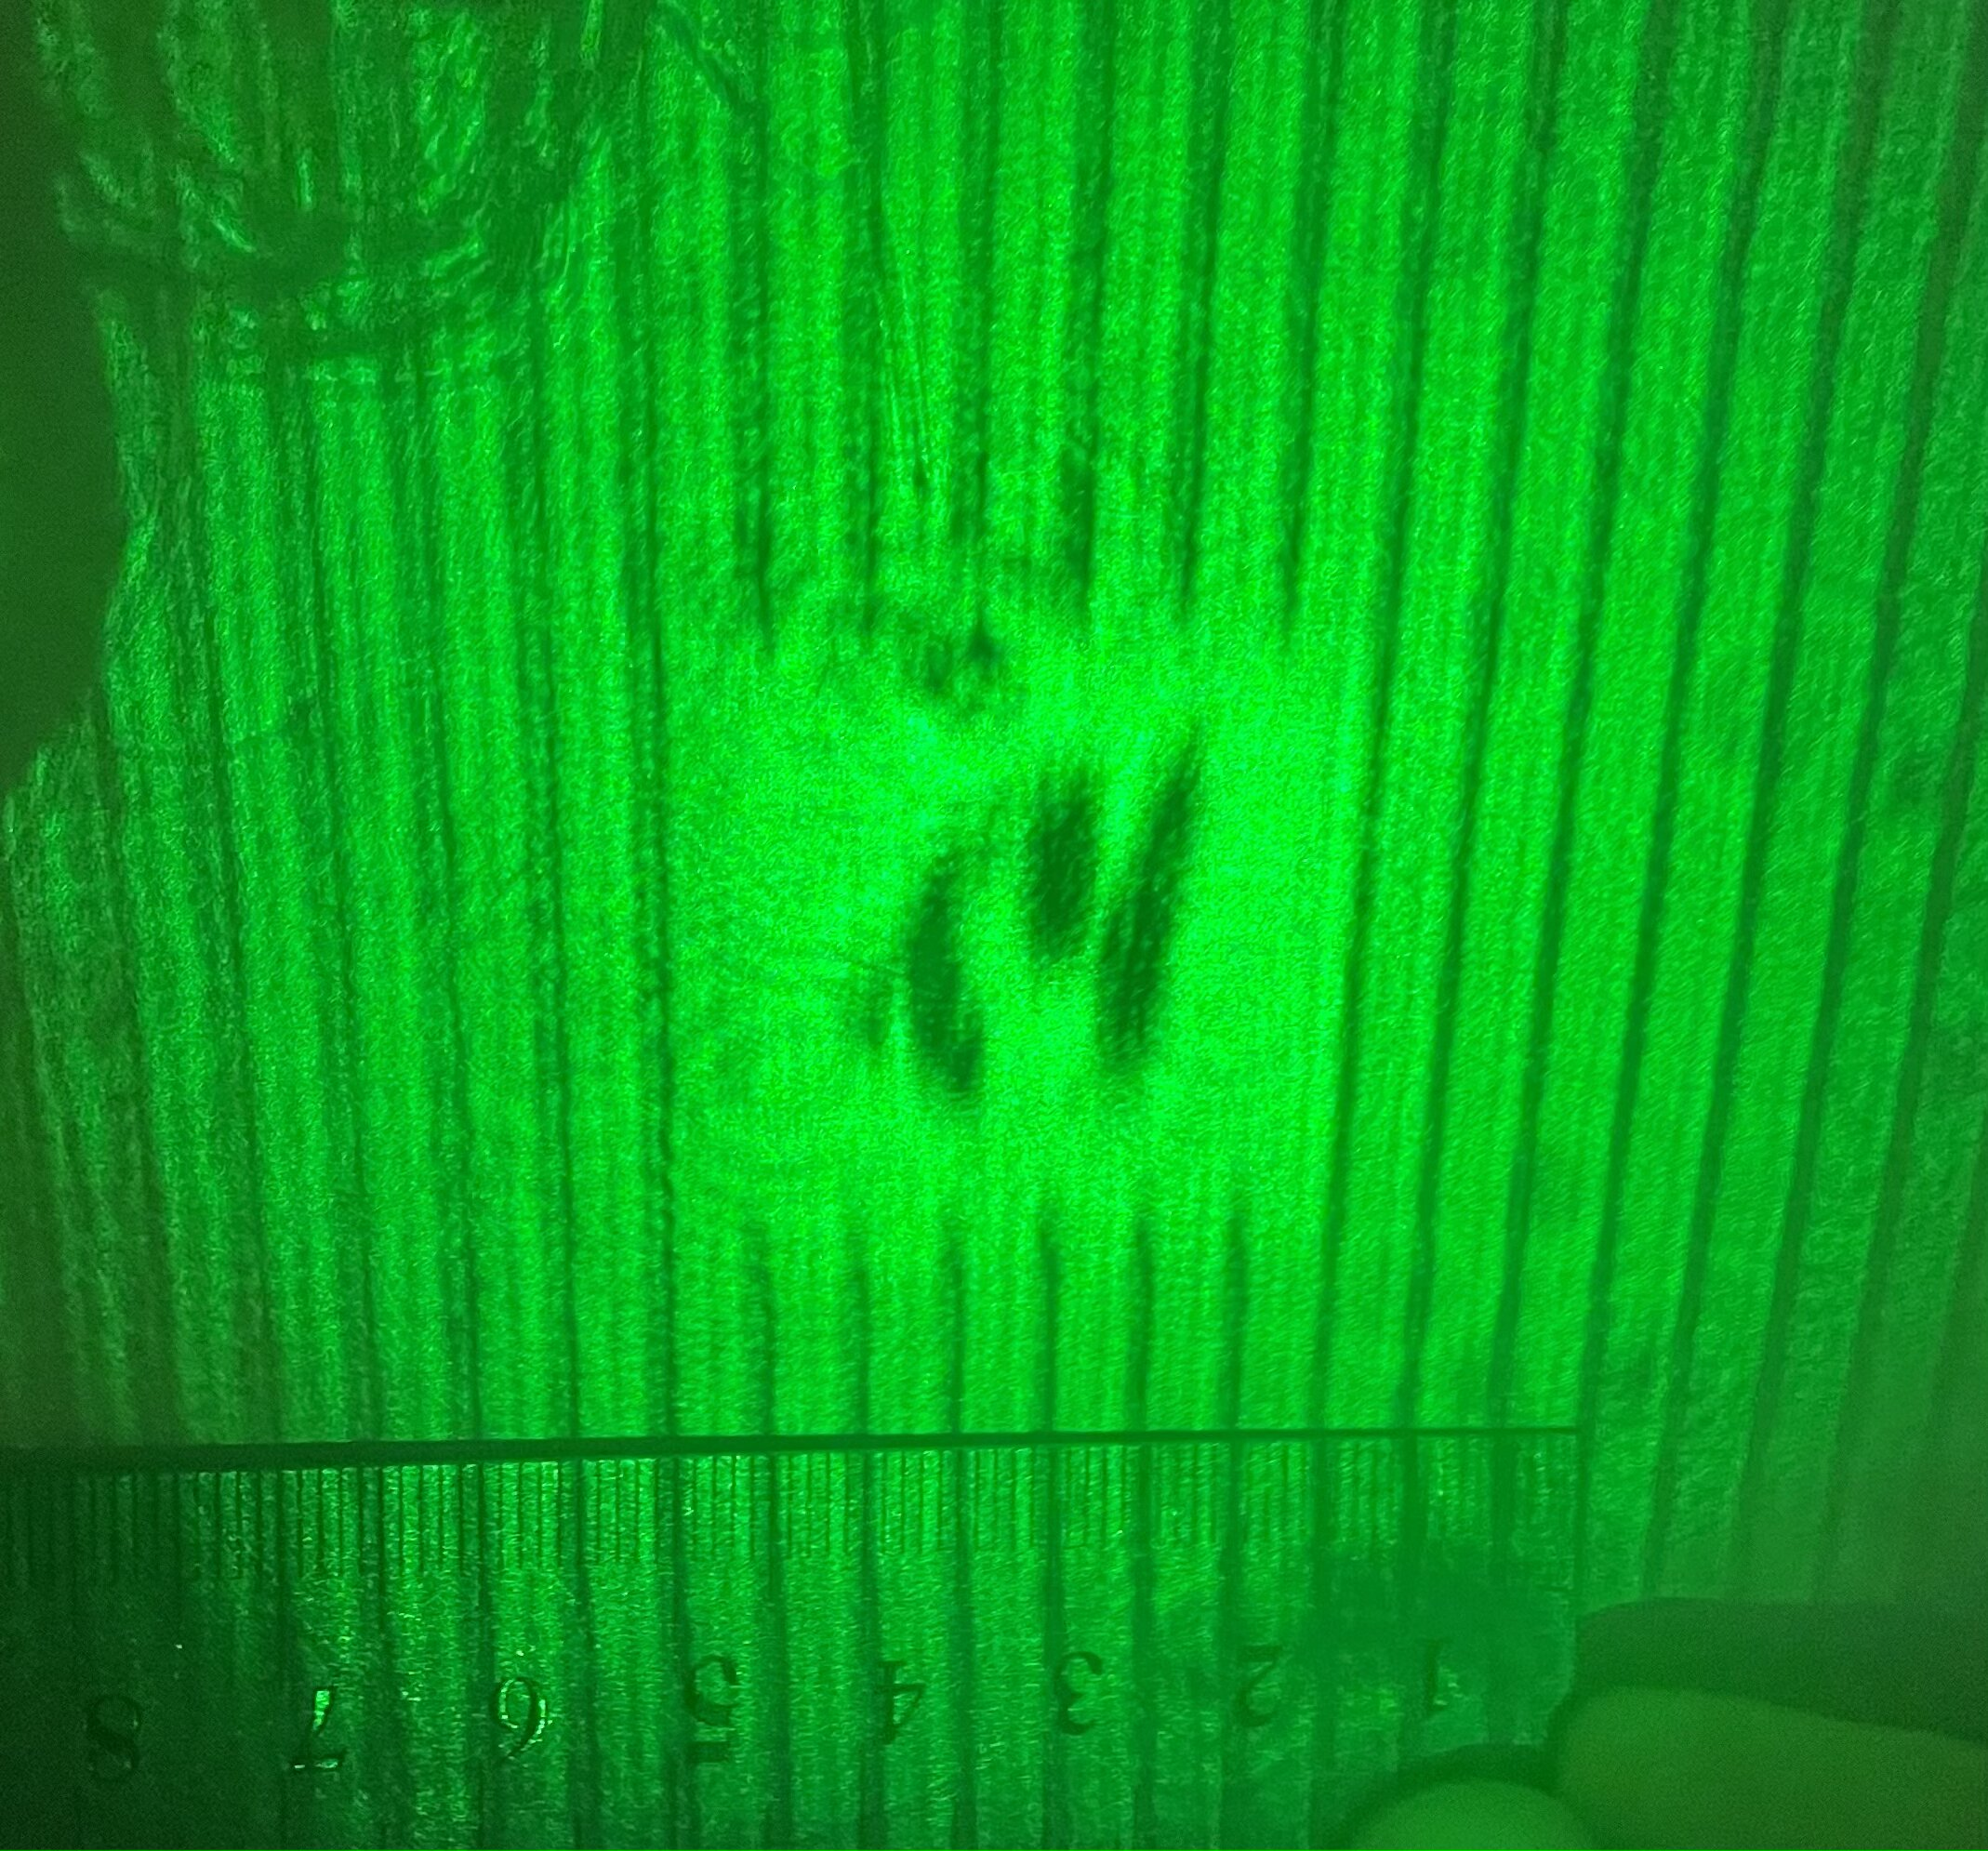
\includegraphics[width=0.75\linewidth]{src/hor.jpeg}
			\caption{Горизонатальная щель}
		\end{figure}



\newpage

    \section*{Вывод}

    По измерениям спектров получилось определить дифракционные углы и по теоретическим формулам рассчитали периоды решеток. Полученные данные сошлись с результатами,  полученными по измерениям увеличенных с помощью микроскопа изображений сеток. Построив график зависимости d = f(1/D), взяв периоды сеток, определённые по спектру мы убедились в справедливости теории Аббе. 

\begin{thebibliography}{9}
	\bibitem{Siv} Сивухин Д. В. \emph{Общий курс физики. Том 4 Оптика}, 2004
	\bibitem{kirich} Кириченко Н.А. \emph{Оптика.}, 2011
	\bibitem{max} \emph{Лабораторный практикум по общей физике. В 3 томах. Том 3. Оптика: учебное пособие} под ред. А. В. Максимычева, М. Г. Никулина
\end{thebibliography}

\end{document}
